\section{Optymalizacja w środowisku \textsc{MATLAB}}

Model matematyczny i znajomość struktury optymalnego sterowania bang-bang wykorzystano do numerycznej optymalizacji wskaźnika jakości określającego jak najszybsze dotarcie do zadanego połozenia równowagi.

Rozwiazywanie równan różniczkowych w środowisku MATLAB odbywało się metodą Rungego-Kutty czwartego rzędu. 

Funkcja \texttt{rk4} rozwiązuje równania stanu "w przód". Parametrami wejściowymi dla funkcji są: punkt początkowy,
wektor sterowań, czasy przełączeń oraz krok dyskretyzacji. Funkcja zwraca rozwiązanie równań stanu oraz
czas. Różniczkowe równania stanu zawarto w funkcji rhs, który jest wywoływany wewnątrz rk4.

Funkcja \texttt{r4k\_inv} rozwiązuje równania sprzężone "wstecz". Parametrami wejściowymi dla funkcji są: rozwiązanie
równań stanu, wektor sterowań, czasy przełączeń, krok dyskretyzacji, punkt docelowy oraz współczynnik ro.
Funkcja zwraca rozwiązanie równań sprzężonych.Różniczkowe równania sprzężone zawarto w funkcji \texttt{rhs\_inv}, 
który jest wywoływany wewnątrz funkcji \texttt{rk4\_inv}.

Funkcja celu (nazwana \texttt{funkcja\_celu\_z\_gradientem}) wykonuje opisane powyżej czynności, a więc rozwiązuje 
równania stanu "w przód" oraz równania sprzężone "wstecz". Następnie wylicza wskaźnik jakości dla danego 
wektora przełączeń. Wskaźnik jakości obliczany jest dla stanu końcowego zgodnie ze wzorem \ref{wskaznik}. 
Największą wagę we wskaźniku jakości przypisano dla położenia oraz prędkości kulki, ponieważ uznano, że 
parametry te powinny być w jak największym stopniu zgodne z oczekiwanymi. Ostatnim etapem w napisanej 
funkcji celu jest obliczenie gradientów wskaźnika jakości dla chwil przełączeń oraz czasy końcowego
zgodnie ze wzorem (...). Parametrami wejściowymi funkcji celu są: punkt początkowy, krok dyskretyzacji,
czasy przełączeń, współczynnik ro, punkt docelowy oraz wektor sterowań. Funkcja celu zwraca obliczoną
wartość wskaźnika jakości oraz wektor gradientów wskaźnika jakości.



\begin{figure}[!htb]
\centering
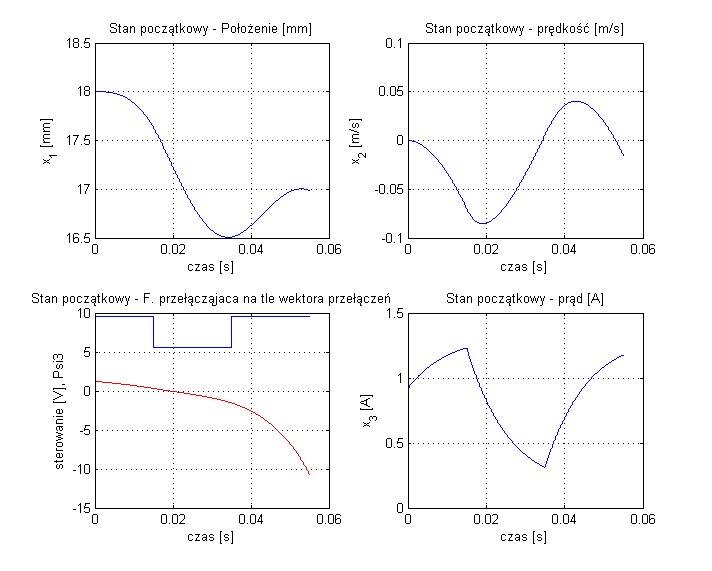
\includegraphics[scale=1]{img/start2.png}
\caption{Rozwiązanie przed optymalizacją z wektorem przełączeń $\tau = [0.015, 0.035, 0.055]$}
\label{rys:start1}
\end{figure}


\begin{figure}[!htb]
\centering
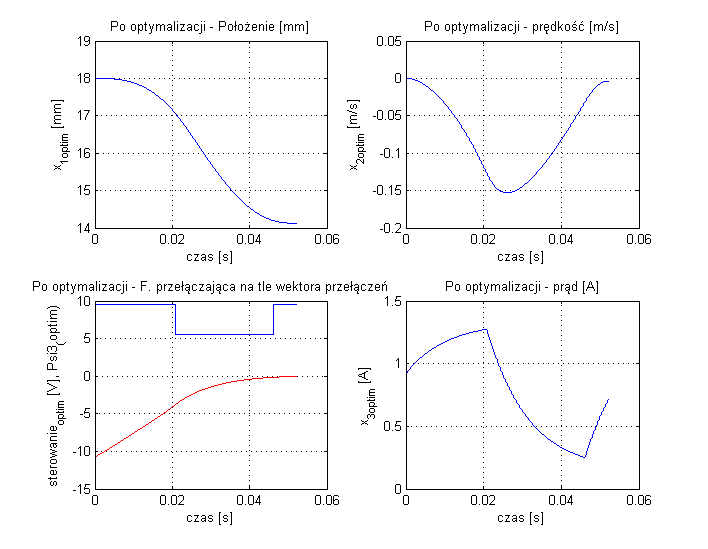
\includegraphics[scale=1]{img/optim2.png}
\caption{Przebieg dla sterowania po optymalizacji}
\label{rys:start1}
\end{figure}

\newpage
\subsection{Wykorzystanie ustawień fmincon()}

Skrypt \texttt{MagLev\_main} jest głównym programem służącym do optymalizacji lewitacji magnetycznej. Na początku
można określić indywidualne czasy przełączeń, wektor sterowań, zadane stany początkowy i końcowy oraz
krok dyskretyzacji. W dalszej części programu rozwiązywane są równania stanu "w przód" i równania
sprzężone "wstecz" dla parametrów początkowych. Rysowane są również wykresy przedstawiające zmienne stanu, 
funkcję sterującą oraz funkcję przełączającą dla warunków początkowych oraz obliczany jest wskaźnik jakości
wraz z gradientem. Optymalizacja początkowego rozwiązania wykonywana jest z użyciem funkcji wbudowanej 
\texttt{fmincon()} w programie Matlab. Dodano ograniczenia nierównościowe, aby zachować odpowiednie wartości czasów
przełączeń. Dodatkowo ustawiono dolną i górną granicę dla szukanych optymalnych czasów przełączeń. Nie 
mogą różnić sie one o wielkość większą niż delta od początkowych czasów przełączeń. Zdecydowano się na to
dodatkowe ograniczenie, ponieważ umożliwiał on szybsze znalezienie sterowania optymalnego przez funkcję
fmincon. Dodatkowo w opcjach funkcji fmincon zastosowano algorytm \quotedblbase \texttt{active-set}\textquotedblright, włączono opcję gradientu
obliczanego w funkcji celu oraz ustawiono ograniczenia na maksymalną liczbę iteracji oraz wywołań funkcji.
Ograniczenia te zastosowano, ponieważ zauważono, że obliczane wyniki są zadowalające dużo wcześniej, niż
funkcja fmincon domyślnie kończy pracę. Ostatnim etapem optymalizacji jest obliczenie i wyświetlenie 
wartości zmiennych stanu, funkcji sterującej i funkcji przełączającej dla znalezionych, zoptymalizowanych
wartości przełączeń. 

\begin{figure}[!htb]
\centering
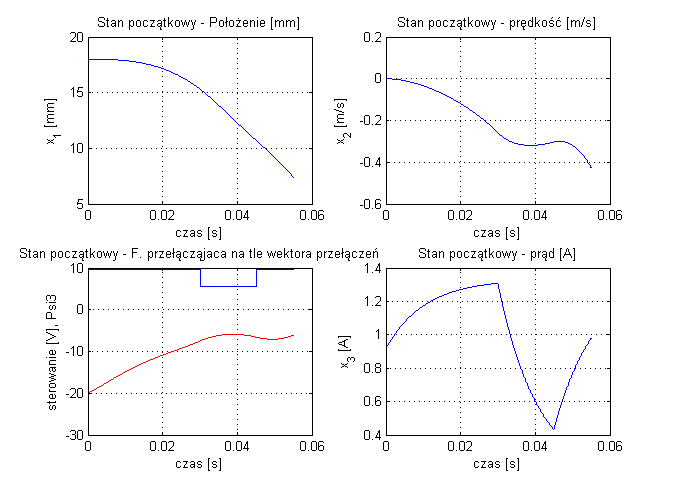
\includegraphics[scale=1]{img/start3.png}
\caption{Rozwiązanie przed optymalizacją z wektorem przełączeń $\tau = [0.03, 0.045, 0.055]$}
\label{rys:start1}
\end{figure}


\begin{figure}[!htb]
\centering
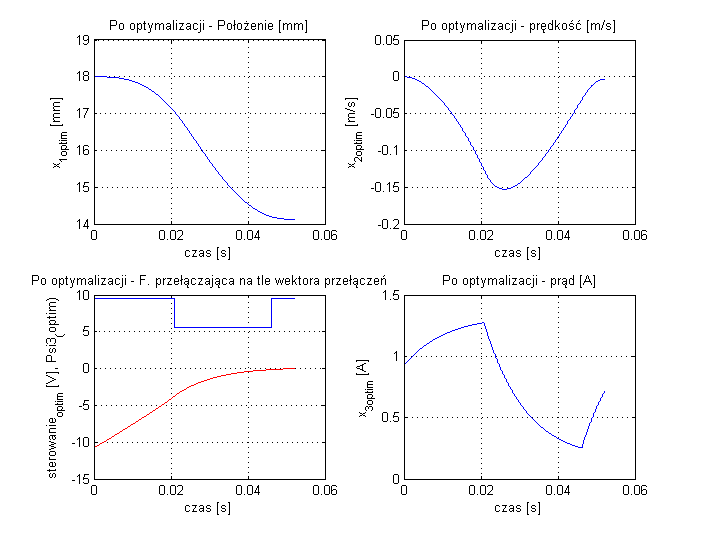
\includegraphics[scale=1]{img/optim3.png}
\caption{Przebieg dla sterowania po optymalizacji, dobrane numerycznie $\tau = [0.7412,  1.6434, 1.8554]$}
\label{rys:start1}
\end{figure}
